\documentclass{endm}
\usepackage{endmmacro}
\usepackage{graphicx}

% The following is enclosed to allow easy detection of differences in
% ascii coding.
% Upper-case    A B C D E F G H I J K L M N O P Q R S T U V W X Y Z
% Lower-case    a b c d e f g h i j k l m n o p q r s t u v w x y z
% Digits        0 1 2 3 4 5 6 7 8 9
% Exclamation   !           Double quote "          Hash (number) #
% Dollar        $           Percent      %          Ampersand     &
% Acute accent  '           Left paren   (          Right paren   )
% Asterisk      *           Plus         +          Comma         ,
% Minus         -           Point        .          Solidus       /
% Colon         :           Semicolon    ;          Less than     <
% Equals        =           Greater than >          Question mark ?
% At            @           Left bracket [          Backslash     \
% Right bracket ]           Circumflex   ^          Underscore    _
% Grave accent  `           Left brace   {          Vertical bar  |
% Right brace   }           Tilde        ~

\newcommand{\Nat}{{\mathbb N}}
\newcommand{\Real}{{\mathbb R}}
\def\lastname{Please list your Lastname here}

\begin{document}

% DO NOT REMOVE: Creates space for Elsevier logo, ScienceDirect logo
% and ENDM logo
\begin{verbatim}\end{verbatim}\vspace{2.5cm}

\begin{frontmatter}

\title{Hoy te convert\'is en (Junior) Data Scientist}

%\author{My Name\thanksref{ALL}\thanksref{myemail}}
\author{Ricardo Colombo}
\author{Diego Santos}
\author{Erik Machicado}
%\address{My Department\\ My University\\ My City, My Country}
\address{Departamento de Computaci\'on\\ Universidad de Buenos Aires\\ C.A.B.A, Argentina}

% \author{My Co-author\thanksref{coemail}}
% \address{My Co-author's Department\\ My Co-author's University\\
%    My Co-author's City, My Co-author's Country} \thanks[ALL]{Thanks
%    to everyone who should be thanked} \thanks[myemail]{Email:
%    \href{mailto:myuserid@mydept.myinst.myedu} {\texttt{\normalshape
%    myuserid@mydept.myinst.myedu}}} \thanks[coemail]{Email:
%    \href{mailto:couserid@codept.coinst.coedu} {\texttt{\normalshape
%    couserid@codept.coinst.coedu}}}

% \begin{abstract}
% This is a short example to show the basics of using the ENDM style
% macro files. Ample examples of how files should look may be found
% among the published volumes of the series at the ENDM home page
% ({\texttt{http://www.elsevier.com/locate/endm}})
% \end{abstract}

\begin{abstract}
El trabajo consiste en aplicar t\'ecnicas de M\'etodos num\'ericos y 
Data Science, en particular Regresiones Lineales y Cuadrados M\'inimos, 
a un gran conjunto de datos reales, buscando identificar modelos 
capaces de predecir comportamientos .
\end{abstract}

\begin{keyword}
Data Science, KPIs, Cuadrados Minimos Lineales (CML)
\end{keyword}

\end{frontmatter}


\section{Introducci\'on}\label{intro}

%Contendrá una breve explicación de la base teórica que fundamenta los métodos involucrados en el trabajo, junto con los métodos mismos. No deben incluirse demostraciones de propiedades ni teoremas, ejemplos innecesarios, ni definiciones elementales (como por ejemplo la de matriz simétrica). En vez de definiciones básicas es conveniente citar ejemplos de bibliografía adecuada. Una cita vale más que mil palabras

En la competitiva industria aeron\'autica la eficiencia de los procesos es vital para mantener la calidad del servicio. Cumplir con el servicio no es algo que solo dependa de la empresa que se contrata, ya que a\~no a a\~no la cantidad de vuelos se multipilica y muchas veces existen variables externas que terminen afectando la puntualidad y calidad del servicio. Por eso es importante contar con m\'etricas que analizen los eventos pasados buscando patrones e intentar prevenirlos o desminuir su impacto en el futuro. Estos indicadores son denominados \textit{Key Performance Indicators} (KPIs).

En este trabajo estudiaremos factores que influyen en la organizaci\'on de las salidas de vuelos para un aeropuerto en particular. Como se mencion\'o anteriormente estad\'isticamente, todos los a\~nos se registran mas vuelos para cualquier aeropuerto, esto requiere una sincronizaci\'on precisa de los tiempos que ocupa un avi\'on dentro del aeropuerto esperando para partir.

Nuestro primer eje de estudio es la evoluci\'on en la cantidad de tr\'afico \'aereo de un aeropuerto, y como la cuota de \textit{market share} se fue concentrando con el correr del tiempo sobre las empresas l\'ideres del segmento. Lo interesante de esta evaluaci\'on es esperamos poder proyectar el crecimiento de tr\'afico sobre el aeropuerto a fin de poder satisfacer la creciente demanda.

El segundo eje de estudio se centra en los factores estacionales que influyen en un vuelo salga en tiempo y forma, es decir estudiaremos la cantidad de retrasos en partidas para un aeropuerto particular, con el objetivo de detectar las estaciones anuales donde el clima pueda afectar el funcionamiento del aeropuerto.

Para la realización del trabajo analizaremos un set de datos reales correspondientes a vuelos realizados en Estados Unidos durante el per\'iodo 1987 - 2008. Y para poder relacionar los casos utilizaremos en los dos ejes el mismo aeropuerto.

Luego relacionaremos los ejes de estudio para estudiar si es posible predecir temporadas de mayor retraso, esperando que sea de utilidad en la programaci\'on de los nuevos vuelos que se incorporán al mercado.


%breve explicacion de metodo
\paragraph{Metodo de Minimos Cuadrados}

Minimos cuadrados es una t\'ecnica de an\'a num\'erico, en la que, dados un conjunto de pares intenta encontrar la funci\'on que mejor aproxime a los datos de acuerdo con el criterio de Error cuadr\'atico medio. En su forma m\'as simple, intenta minimizar la suma de los cuadrados de las diferencias entre los puntos generados por la funci\'on de aproximaci\'on y los que corresponden a los datos. CML es el caso en el que se usa a las rectas para la aproximaci\'on osea $y = ax + b$, adem\'as la generalizaci\'on del m\'etodo propone encontrar la funci\'on que mejor aproxima de la forma $y = a_1f_1(x) + \dots + a_Kf_K(x)$ y que no es necesario que las funciones $f$ sean lineales pero si que $y$ sea una combinaci\'on lineal de ellas. Para mas informacion consultar  \cite{bf} (seccion 8.1)

\section{Desarrollo}
	%Deben explicarse los métodos numéricos que utilizaron y su aplicación al problema concreto involucrado en el trabajo práctico. Se deben mencionar los pasos que siguieron para implementar los algoritmos, las dificultades que fueron encontrando y la descripción de cómo las fueron resolviendo. Explicar también cómo fueron planteadas y realizadas las mediciones experimentales. Los ensayos fallidos, hipótesis y conjeturas equivocadas, experimentos y métodos malogrados deben figurar en esta sección, con una breve explicación de los motivos de estas fallas (en caso de ser conocidas).

En an\'alisis de las m\'etricas que proponemos esta centradado en el aeropueto \textit{JFK}. Tomandolo como referencia en nuestro primer eje estudiaremos la evoluci\'on de la cantidad de vuelos de ese aeropuerto, y veremos cual es la cuota de mercado de las dos empresas reconocidas mundialemente \textit{Delta} y \textit{United Airlines} y su evoluci\'on a traves de los a\~nos. En el segundo eje estudiaremos la cantidad de demoras que se producen por condiciones climaticas. Tomando como definici\'on de demora, un vuelo que sale al menos 15 minutos despues de su horario programado. El objetivo de este caso es identificar temporadas c\'iciclas donde las condiciones clim\'aticas afectan el comportamiento normal del aeropuerto.

Para finalizar intentaremos probar si hay alguna relaci\'on entre el crecimiento de los vuelos y la cantidad de demoras estacionales generadas por el clima.

Para la realizaci\'on del estudio implementamos una serie de algoritmos utilizando el lenguaje \textit{Python}. En la primer etapa procesamos el data set inicial filtrando los registros que nos interesa estudiar y los agrupamos por mes. Luego para entrenar nuestra soluci\'on propuesta tomamos un subconjunto de meses de los datos conocidos de forma random, ejecutamos el proceso para una cantidad \textit{n} tambi\'en random y validamos los resultados obtenidos utilizando la t\'ecnica de \textit{Coss-Validation}. Qued\'andonos con los que min\'imizen el error. Para evitar caer en el conocido overfitting elegiremos distintos subconjuntos del training para hallar los coeficientes de la aproximacion lineal.

Luego el siguiente paso es ver como con los datos entrenados nuestras funciones que tan bien aproximan al valor real e intentar predecir el comportamiento futuro.

\subsection{Crecimiento de vuelos}

Luego de analizar los resultados vemos que hay un crecimiento relativamente lineal de la cantidad de vuelos, con excepciones donde crece de forma exponencial.

Además con el correr de los años la cuota de mercado de ambas empresas crece, pero una m\'as que la otra.


\subsection{Demoras Clim\'aticas}

Luego de analizar los resultados, propusimos funciones que intenten aproximar de forma adeacuada a los datos reales. En primera instancia intentamos con funciones polin\'omicas, pero el modelo generado distaba bastante de lo real. Ya que los datos tienen un comportamiento c\'iclico.

Encontramos que la mejor forma de aproximaci\'on es una combinaci\'on de funciones trigonom\'etricas sobre prolinomios.



\section{Resultados}

	\begin{center}
	\caption{figura 1}
	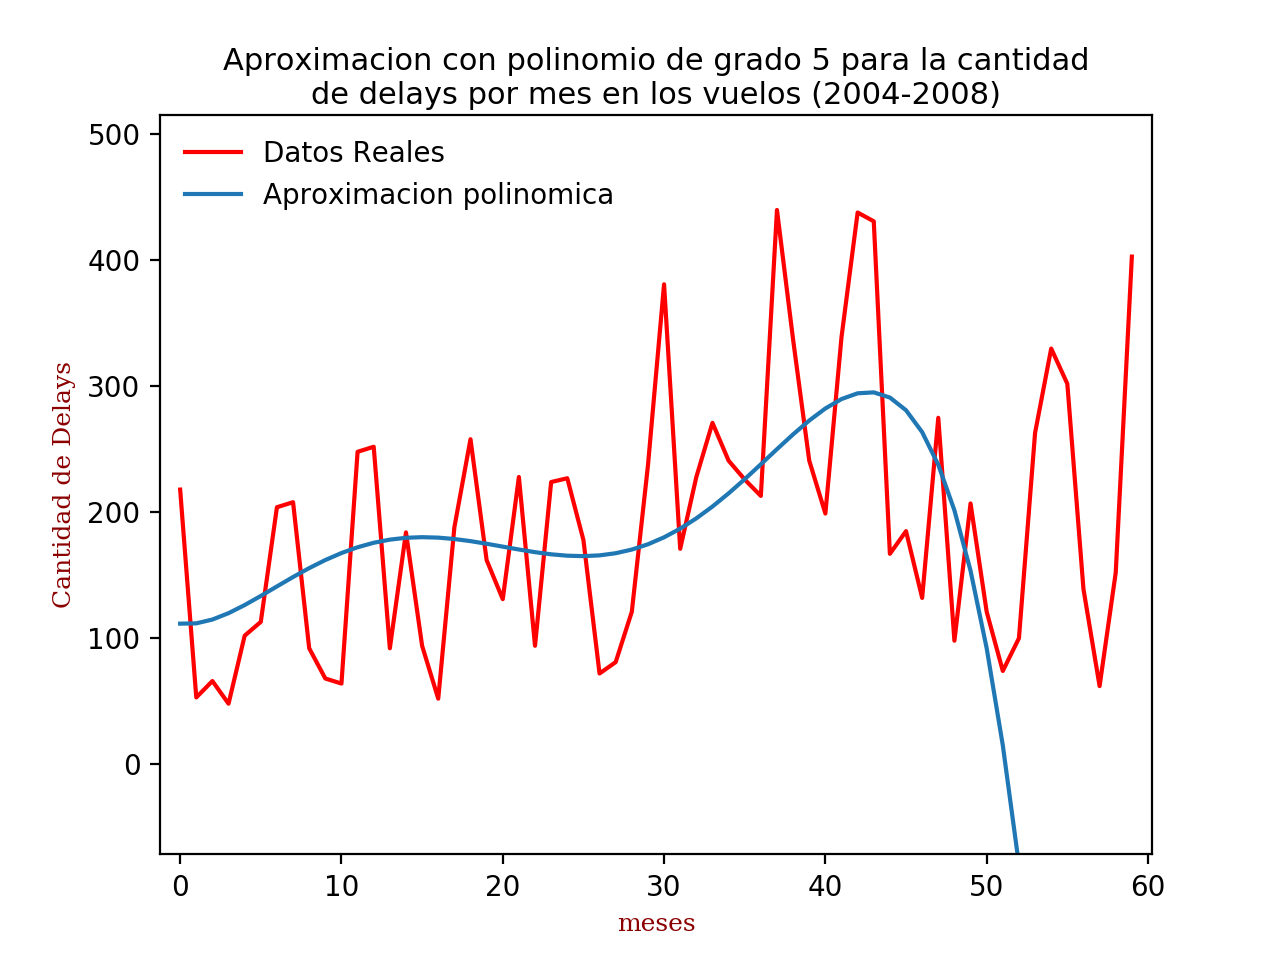
\includegraphics[scale=0.7]{imagenes/delaysPolinomio.png}
	\end{center}

	\begin{center}
	\caption{figura 2}
	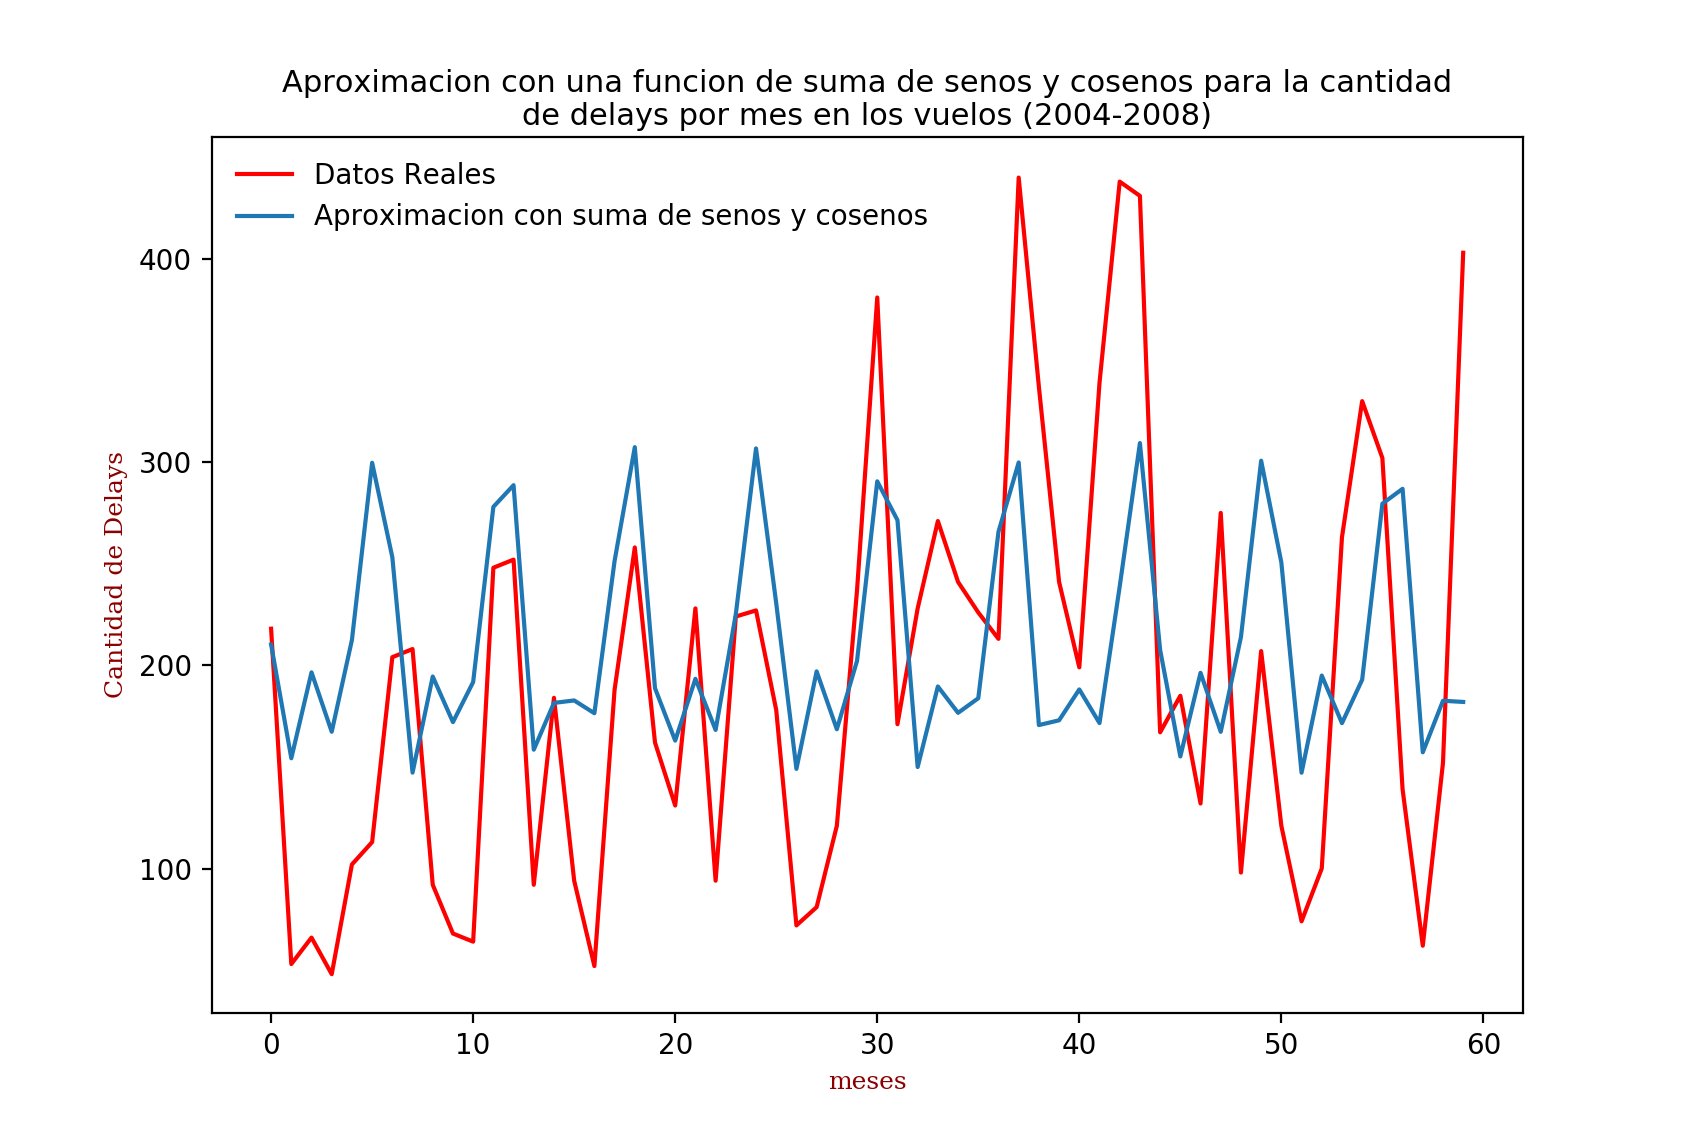
\includegraphics[scale=0.6]{imagenes/senosCosenos.png}
	\end{center}

	\begin{center}
	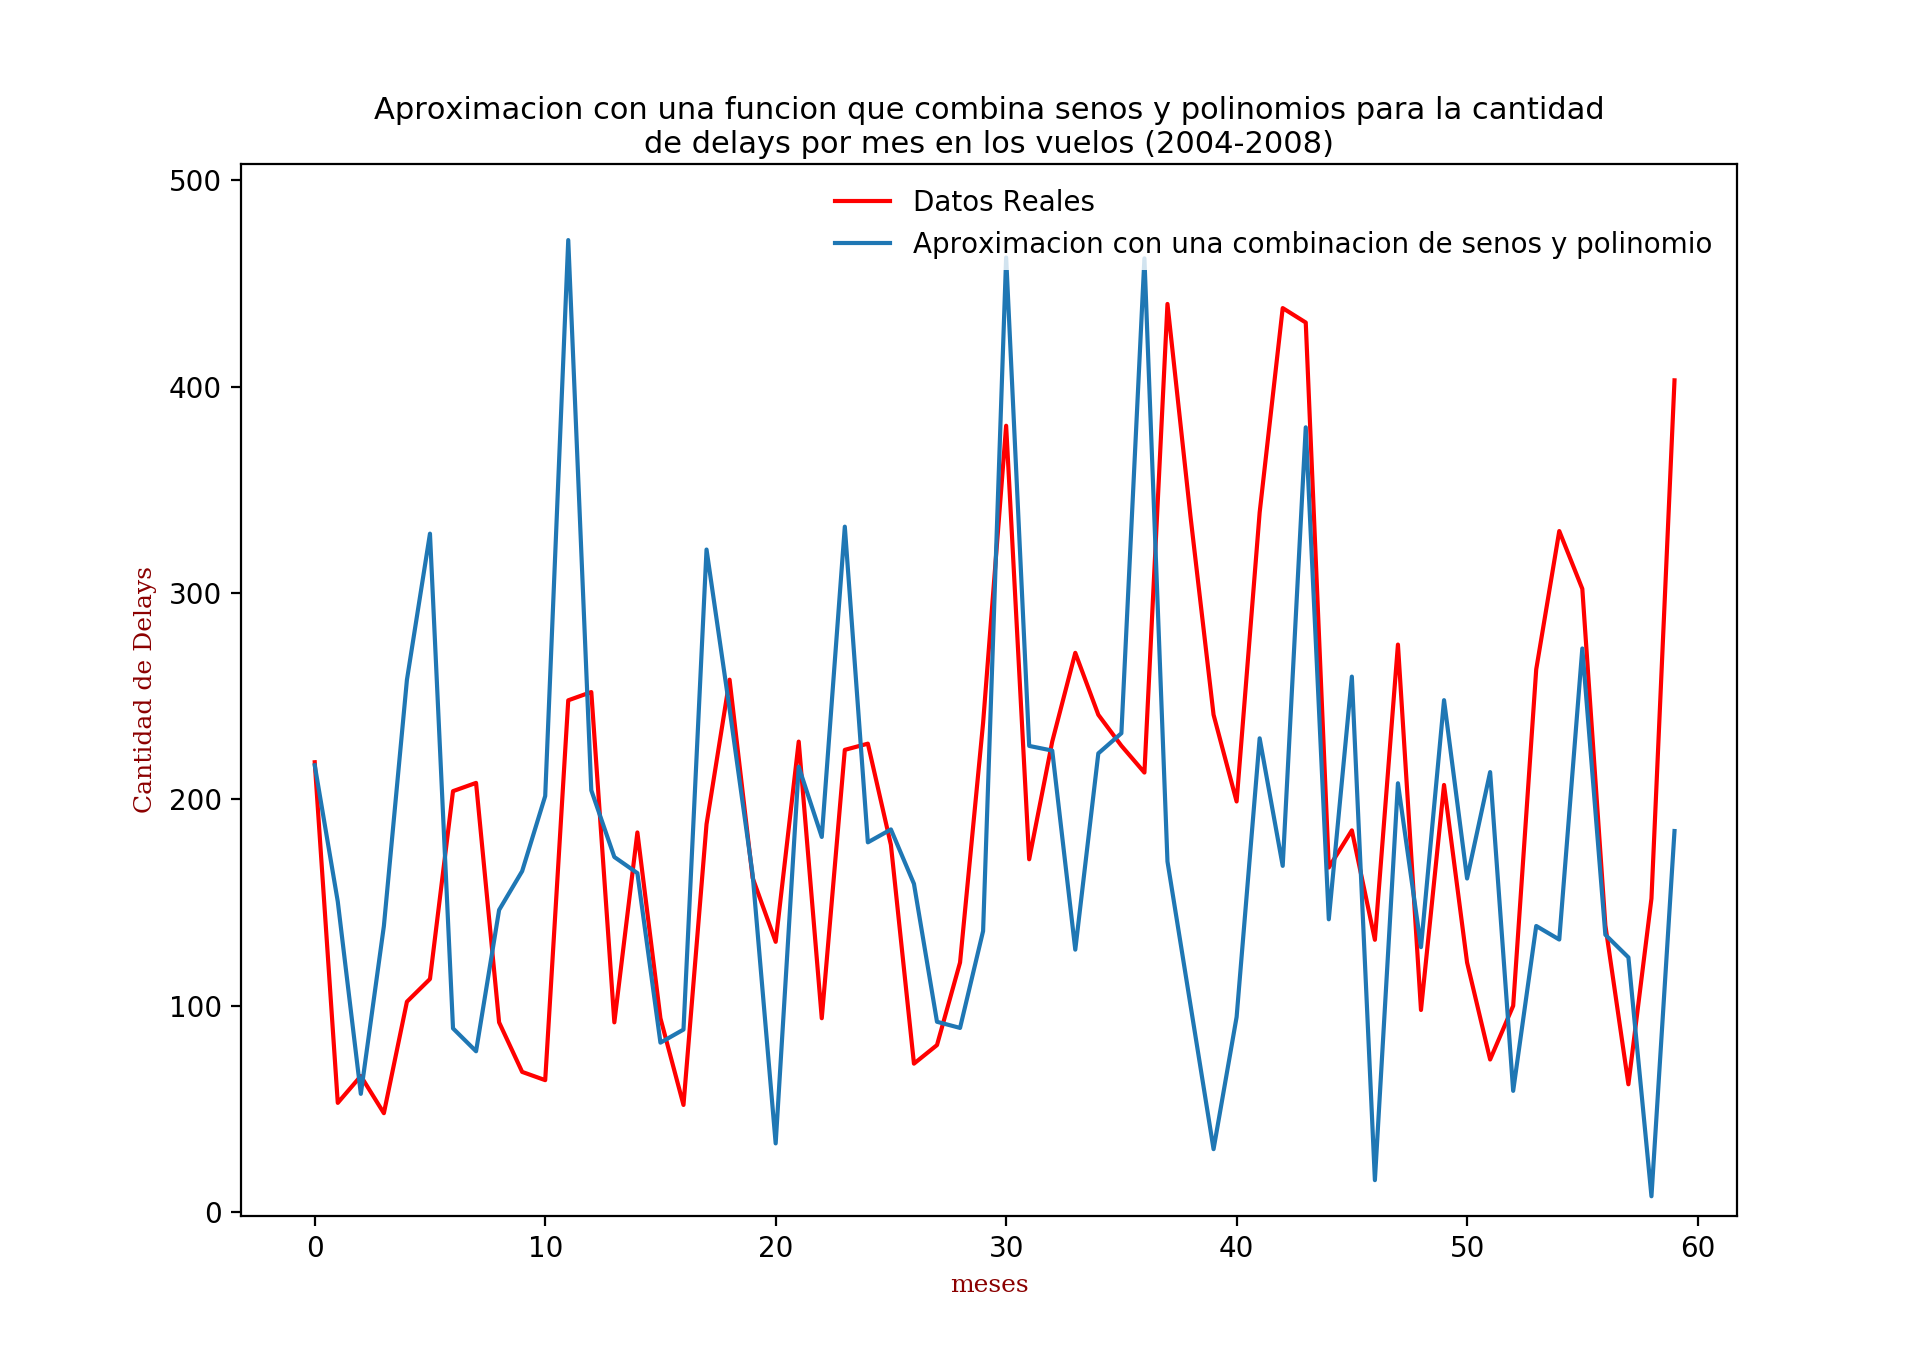
\includegraphics[scale=0.5]{imagenes/polinomioysenos.png}
	\end{center}

	\begin{center}
	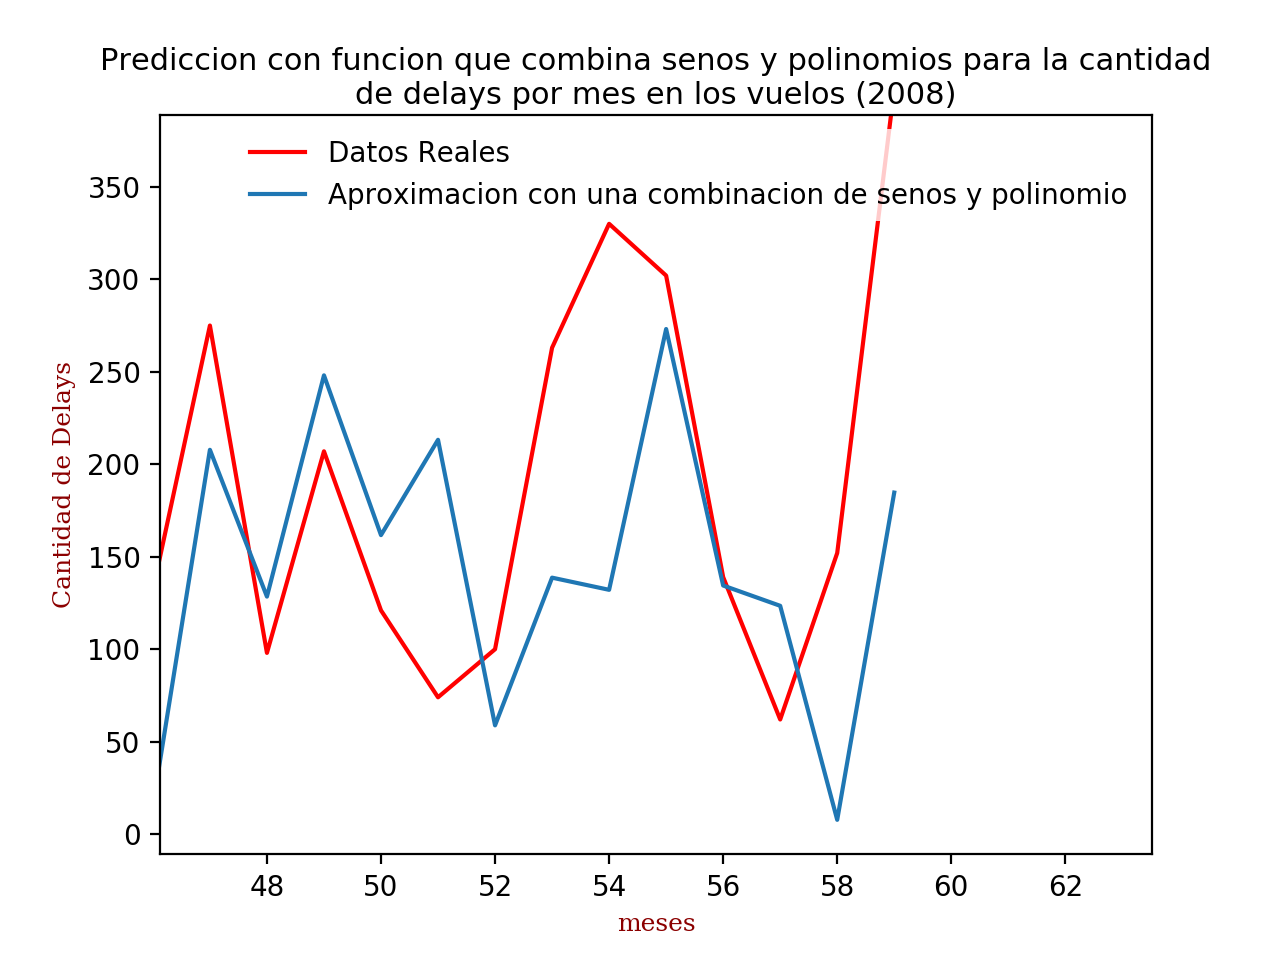
\includegraphics[scale=0.8]{imagenes/delays2008.png}
	\end{center}

\section{Discusi\'on}
	%Hablar de las limintaciones de cada tipo de funcion 
	Durante la experimentacion con la familias de polinomios usadas para el metodo se encontro que si bien en los meses de training se aproximaba bien afuera de ese periodo se aleja de los datos reales, como esta ilustrado en el grafico de la figura 1 que utiliza los datos del periodo 2004-2007 para predecir 2008 (apartir del mes 48) despues de discutirlo entendimos que la cantida de picos que tiene un polinomio esta limitada por el grado del mismo, pues son las raices del polinomio derivado y estas a lo sumo son tantas como el grado del polinomio derivado por eso fuera del periodo usado como training no se generan nuevos picos apesar que los datos reales si los tienen. Cuando usamos senos y cosenos como familias de funciones para el metodo nos encontramos con que estas estaban acotadas como lo estan los senos y cosenos, y no podian crecer si los datos lo hacian como lo muestra la figura 2





\section{Conclusiones}
	%Hablar sobre la funcion final que escogimos y como reune los que queremos de la dos funciones




\begin{thebibliography}{10}\label{bibliography}
  
\bibitem{bf} Burden, R. L., and J. D. Faires, ``An\'alisis num\'erico,
'' Math. Surveys \textbf{7}, Amer. Math. Soc.,
  Providence, R.I., 1961.
  
\bibitem{d} ASA Section on Statistical Computing. 2009 data expor competition, URL:
  \href{http://stat-computing.org/dataexpo/2009/the-data.html}
  {\texttt{http://stat-computing.org/dataexpo/2009/the-data.html}}.

\end{thebibliography}

\end{document}
